\documentclass{beamer}
\usepackage{lipsum,enumerate,framed,setspace,multirow,paralist,sgamevar,pstricks,amssymb,amsfonts,amsmath,color,egameps,graphicx,parskip,tikz,pgfplots,sgamevar,changepage,soul,framed,wrapfig} 
\usepackage{sansmathaccent}
\pdfmapfile{+sansmathaccent.map}
%%%%%%%%%%%%
% Template %
%%%%%%%%%%%%
% Page dimension
\setbeamertemplate{itemize items}{\scriptsize\textbullet}
\setbeamercovered{invisible}
% Page dimension
\paperwidth=18cm
\paperheight=8cm
\textwidth=14cm
\oddsidemargin=-1cm
\topmargin=0cm
\headsep=5pt
\marginparsep=1cm
\marginparwidth=1cm
\voffset=-2cm
\hoffset=0cm
\setlength{\parindent}{0pt}
\setlength{\parskip}{12pt}
\setbeamertemplate{frametitle}{\insertframetitle} 
\setbeamercolor{palette primary}{fg=black}



\usetikzlibrary{tikzmark}




\begin{document}

\begin{frame}[t]
\begin{center}
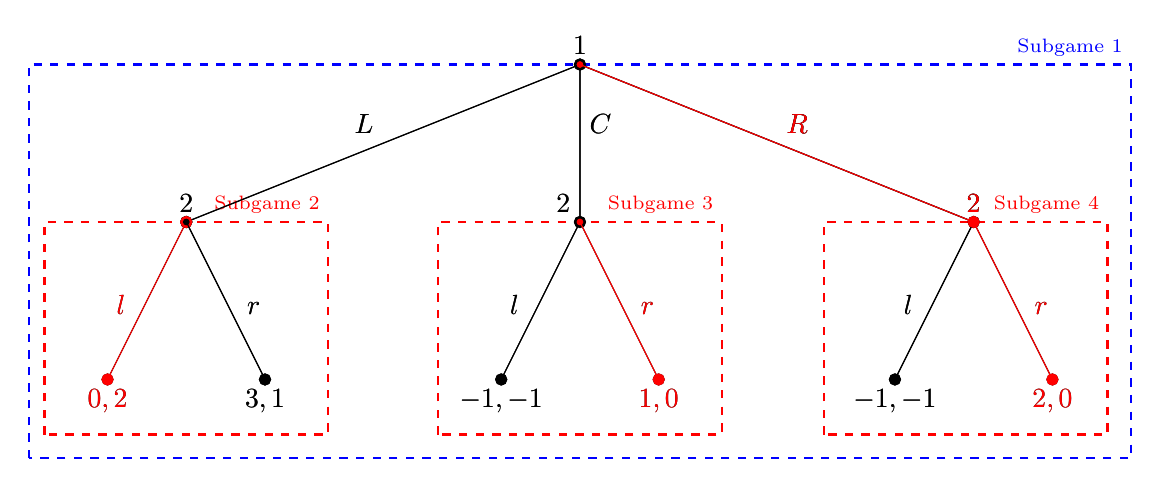
\begin{tikzpicture}

\coordinate (1) at (0,1);
\coordinate (2a) at (-5,-1);
\coordinate (2b) at (0,-1);
\coordinate (2c) at (5,-1);



%Left branch
\filldraw (1) circle [fill=none,radius=2pt]-- (2a)  node[anchor=south,pos=1] {2} node[anchor=south,pos=0]{1}  node[anchor=south east,pos=.5] {$L$} circle (2pt) {};
\filldraw (2a) circle (2pt) -- (-6,-3)  node[pos=.65,anchor=south east]{$l$} circle (2pt) node[anchor=north]  {$0,2$};
\filldraw (2a) circle (1pt) -- (-4,-3) node[pos=.65,anchor=south west]{$r$} circle (2pt) node[anchor=north]  {$3,1$};

%Center branch
\filldraw (1) circle (1pt) -- (2b)  node[anchor=south east,pos=1] {2} node[anchor=south west,pos=.5] {$C$} circle (2pt) {} ;
\filldraw  (2b) circle (1pt) -- (-1,-3)  node[pos=.65,anchor=south east] {$l$}circle (2pt)  node[anchor=north] {$-1,-1$};
\filldraw (2b) circle (1pt) -- (1,-3) node[pos=.65,anchor=south west] {$r$} circle (2pt)  node[anchor=north] {$1,0$};

%Right branch
\filldraw (1) circle (1pt) -- (2c)  node[anchor=south,pos=1] {2} node[anchor=south west,pos=.5]   {$R$} circle (2pt) {};
\filldraw  (2c) circle (1pt) -- (4,-3)  node[pos=.65,anchor=south east]{$l$}circle (2pt)  node[anchor=north] {$-1,-1$};
\filldraw (2c) circle (1pt) -- (6,-3) node[pos=.65,anchor=south west]{$r$} circle (2pt)  node[anchor=north] {$2,0$};
%Subgames\
{\scriptsize
\pause\draw[fill=none,thick, dashed,draw=blue]  (-7,-4) rectangle++(14,5) node[pos=1, anchor=south east] {{\color{blue} Subgame 1}} ;
\pause\draw[fill=none,thick, dashed,draw=red]  (-6.8,-3.7) rectangle++(3.6,2.7)  node[pos=1, anchor=south east] {{\color{red} Subgame 2}} ;
\pause\draw[fill=none,thick, dashed,draw=red]  (-1.8,-3.7) rectangle++(3.6,2.7)  node[pos=1, anchor=south east] {{\color{red} Subgame 3}} ;
\pause\draw[fill=none,thick, dashed,draw=red]  (3.1,-3.7) rectangle++(3.6,2.7) node[pos=1, anchor=south east] {{\color{red} Subgame 4}} ;
}

\pause
%Left branch
\filldraw (1) circle [fill=none,radius=2pt]-- (2a)  node[anchor=south,pos=1] {2} node[anchor=south,pos=0]{1}  node[anchor=south east,pos=.5] {$L$} circle (2pt) {};
\filldraw[red] (2a) circle (2pt) -- (-6,-3)  node[pos=.65,anchor=south east]{$l$} circle (2pt) node[anchor=north]  {$0,2$};
\filldraw (2a) circle (1pt) -- (-4,-3) node[pos=.65,anchor=south west]{$r$} circle (2pt) node[anchor=north]  {$3,1$};
\pause

%Center branch
\filldraw (1) circle (1pt) -- (2b)  node[anchor=south east,pos=1] {2} node[anchor=south west,pos=.5] {$C$} circle (2pt) {} ;
\filldraw  (2b) circle (1pt) -- (-1,-3)  node[pos=.65,anchor=south east] {$l$}circle (2pt)  node[anchor=north] {$-1,-1$};
\filldraw[red] (2b) circle (1pt) -- (1,-3) node[pos=.65,anchor=south west] {$r$} circle (2pt)  node[anchor=north] {$1,0$};
\pause
%Right branch
\filldraw (1) circle (1pt) -- (2c)  node[anchor=south,pos=1] {2} node[anchor=south west,pos=.5]   {$R$} circle (2pt) {};
\filldraw  (2c) circle (1pt) -- (4,-3)  node[pos=.65,anchor=south east]{$l$}circle (2pt)  node[anchor=north] {$-1,-1$};
\filldraw[red] (2c) circle (1pt) -- (6,-3) node[pos=.65,anchor=south west]{$r$} circle (2pt)  node[anchor=north] {$2,0$};

\pause 
%Right branch
\filldraw[red] (1) circle (1pt) -- (2c)  node[anchor=south,pos=1] {2} node[anchor=south west,pos=.5]   {$R$} circle (2pt) {};

%Information Set
%\draw [dashed] (0,-1) --(-5,-1) node[pos=.5, anchor=south]{2}; 
%\draw[opacity=0.15,fill=blue, rounded corners] (-3.5, -1.25) rectangle (3.5, -.75) {};
\end{tikzpicture} 
\end{center}
 \end{frame}
 \end{document}